\chapter{Study and realization of the Sprint 1}
\minitoc
\newpage


\setcounter{secnumdepth}{2} % Resume counting the sections for the toc with a depth of 2 (Sections and sub-sections)
% ----------------------------------- SECTIONS (v) ----------------------------------- %
% ----------------------- Functional Requirements ----------------------- %
\section{Backlog of the sprint}
The first sprint was centered on system access and user profile management. Key functionalities like signup, login/logout, and profile management were developed, laying the groundwork for future complex features and ensuring a secure, personalized user experience.

\begin{table}[H]
    \renewcommand{\arraystretch}{1.5}%
    \caption{Sprint 1 Backlog}
    \centering
    \medskip
    \small
    \begin{tabularx}{1.2\textwidth} {
            | >{\hsize=0.8\hsize\raggedright\arraybackslash}X
            | >{\hsize=0.8\hsize\raggedright\arraybackslash}X
            | >{\hsize=1.9\hsize\raggedright\arraybackslash}X
            | >{\hsize=0.5\hsize\raggedright\arraybackslash}X |}
        \hline
        \rowcolor{primary} \textbf{User Story}                                                                              & \textbf{Subtask}                                                                                        & \textbf{Description}                                                                                                                     & \textbf{Estimated Time} \\
        \hline
        As an HR Manager, I want to sign up and create my profile so that I can access the system                           & 1.1 Design and implement the signup process                                                             & Develop a signup page with required fields and necessary backend functionality to register and store the new user's data in the database & 3 days                  \\
        \hline
                                                                                                                            & 1.2 Design and implement the profile creation process                                                   & Implement functionality to allow users to input their profile details post signup, and store this information in the database            & 2 days                  \\
        \hline
        As an HR Manager, I want to login into the system so that I can access the features                                 & 2.1 Design and implement the login process                                                              & Develop a login page and backend functionality to authenticate the user's credentials and grant access                                   & 2 days                  \\
        \hline
        As an HR Manager, I want to be able to update my profile information in the account settings and delete the account & 3.1 Develop a feature that allows HR Managers to update their profile information or delete the account & Implement functionality in the user's account settings to allow them to update their profile details or delete their account             & 3 days                  \\
        \hline
                                                                                                                            & 3.2 Integrate this feature into the system                                                              & Include this functionality in the overall system, ensure it interacts correctly with other system features and data                      & 2 days                  \\
        \hline
    \end{tabularx}
    \normalsize
\end{table}




\newpage
\section{Functional Specification}
In this sub-section, we present the analysis phase that answers the question “what does the system do”. The answer to this question is translated by the presentation of the diagram of the use cases and the textual description of each of them

\subsection{Use Case Diagram}
The use case would typically include the following main actors and their interactions with the system :

\begin{figure}[H]
    \centering
    \makebox[\textwidth]{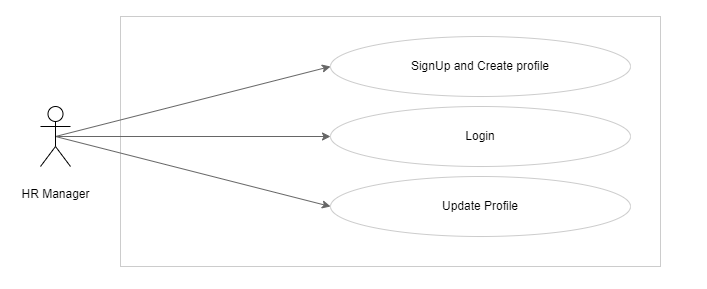
\includegraphics[width=\linewidth]{src/assets/images/HRMUseCase1.drawio.png}}
    \caption{ Use Case Diagram For Sprint 1 }
    \label{fig:Sprint1_UseCaseDiagram}
\end{figure}

\subsection{Textual Description of the Use Cases}

\subsubsection{\underline{Use Case 1 : Sign up and Create Profile}}
In this use case, an HR Manager who is new to the system needs to sign up and create a profile. This involves navigating to the signup page, filling in all necessary personal and company details, such as name, email, password, company name, job role, and other details. Once the form is submitted, the system will validate the provided information. If everything is valid, the system will create a new profile for the HR Manager, and they will be automatically logged into the system.

\newpage
\begin{table}[H]
    \renewcommand{\arraystretch}{1.5}%
    \caption{Use Case: Signup and Profile Creation}
    \centering
    \medskip
    \begin{tabularx}{\textwidth} {
            | >{\hsize=0.5\hsize\raggedright\arraybackslash}X
            | >{\hsize=1.5\hsize\raggedright\arraybackslash}X |}
        \hline
        \textbf{Primary Actor} & HR Manager \\
        \hline
        \textbf{Preconditions} & The HR Manager is on the signup page. \\
        \hline
        \textbf{Postconditions} & The HR Manager has successfully created a profile and can now access the system. \\
        \hline
        \textbf{Main Success Scenario} & 1. The HR Manager navigates to the signup page. \\
        & 2. The HR Manager fills in all necessary personal and company details. \\
        & 3. The HR Manager submits the form. \\
        & 4. The system validates the information, creates a new profile, and logs the HR Manager into the system. \\
        \hline
        \textbf{Alternative Scenarios} & The HR Manager fills in an email address that is already in use. The system displays an error message, and the HR Manager needs to provide a different email address. \\
        \hline
    \end{tabularx}
\end{table}


\subsubsection{\underline{Use Case 2 : Login }}
Once an HR Manager has created a profile, they will need to log in to access the system's features. This use case starts with the HR Manager navigating to the login page and entering their credentials, which are the username (or email) and password they set when they signed up. Once these are submitted, the system verifies the credentials. If the credentials are correct, the HR Manager is logged into the system.

\begin{table}[H]
    \renewcommand{\arraystretch}{1.5}%
    \caption{Use Case: Login}
    \centering
    \medskip
    \begin{tabularx}{\textwidth} {
            | >{\hsize=0.5\hsize\raggedright\arraybackslash}X
            | >{\hsize=1.5\hsize\raggedright\arraybackslash}X |}
        \hline
        \textbf{Primary Actor} & HR Manager \\
        \hline
        \textbf{Preconditions} & The HR Manager has already signed up and created a profile. \\
        \hline
        \textbf{Postconditions} & The HR Manager has successfully logged into the system. \\
        \hline
        \textbf{Main Success Scenario} & 1. The HR Manager navigates to the login page. \\
        & 2. The HR Manager enters their credentials (username/email and password). \\
        & 3. The system verifies the credentials and logs the HR Manager into the system. \\
        \hline
        \textbf{Alternative Scenarios} & The HR Manager enters incorrect credentials. The system displays an error message, and the HR Manager needs to try again. \\
        \hline
    \end{tabularx}
\end{table}


\subsubsection{\underline{Use Case 3 : Update Profile or Delete Account }}
At any point, the HR Manager might need to update their profile information or even delete their account entirely. In this use case, the HR Manager, who is already logged in to the system, navigates to the account settings page. To update their profile, they need to edit the necessary information fields and save the changes. The system will confirm the update once it's successful. On the other hand, to delete their account, they need to click on the "delete account" button and confirm the decision. The system will then delete the account.

\begin{table}[H]
    \renewcommand{\arraystretch}{1.5}%
    \caption{Use Case: Update Profile or Delete Account}
    \centering
    \medskip
    \begin{tabularx}{\textwidth} {
            | >{\hsize=0.5\hsize\raggedright\arraybackslash}X
            | >{\hsize=1.5\hsize\raggedright\arraybackslash}X |}
        \hline
        \textbf{Primary Actor} & HR Manager \\
        \hline
        \textbf{Preconditions} & The HR Manager is already logged into the system. \\
        \hline
        \textbf{Postconditions} & The HR Manager has successfully updated their profile or deleted their account. \\
        \hline
        \textbf{Main Success Scenario} & 1. The HR Manager navigates to the account settings page. \\
        & 2. To update the profile, the HR Manager edits the necessary information and saves the changes. The system confirms the update. \\
        & 3. To delete the account, the HR Manager clicks the "delete account" button, confirms the decision, and the system deletes the account. \\
        \hline
        \textbf{Alternative Scenarios} & - The HR Manager attempts to save invalid information (e.g., an improperly formatted email address). The system displays an error message, and the HR Manager needs to correct the information. \\
        & - The HR Manager requests to delete the account but then cancels the request. The system cancels the deletion process. \\
        \hline
    \end{tabularx}
\end{table}



\section{Design} 
In this sub-section, we will present the different detailed Activity Diagrams + Sequence diagrams for the first sprint.

\subsection{Detailed Activity Diagrams}

A detailed activity diagram allows a comprehensive representation of the processes and interactions within our system in a sequential order. 
It provides a graphical illustration of the workflow of individual steps within a use case, which can aid in understanding the functionality of the system from a user's perspective. Below, we present the activity diagrams of the detailed workflows of the user stories in the first sprint. 
These diagrams visually represent the flow of control from one activity to another and show the various decision paths that exist in the progression of events contained in the use case.

\subsubsection{Use Case 1: Sign Up and Create Profile} 


\begin{figure}[H]
    \centering
    \makebox[\textwidth]{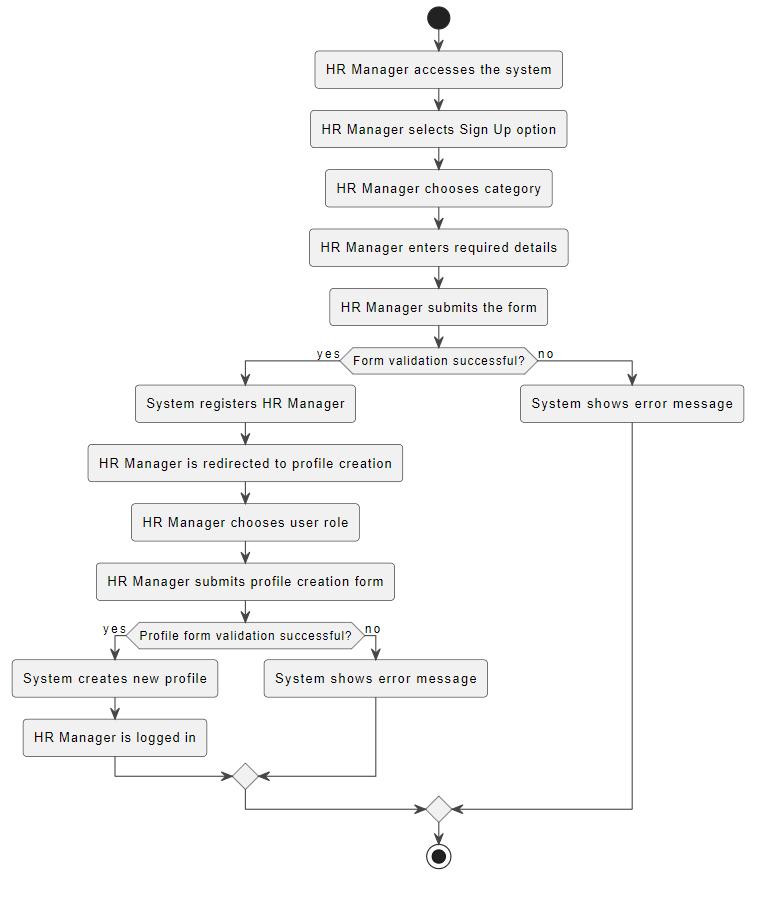
\includegraphics[width=\linewidth]{src/assets/images/sprint1UseCase1ActivityDiagram.PNG}}
    \caption{ Activity Diagram for the Sign Up and Create Profile Use-Case }
    \label{fig:UseCase1_Activity_Diagram}
\end{figure}

\subsection*{Description}
The activity diagram shows the sequence of steps a new HR Manager would take to register in the system. The process begins with the HR Manager initiating the sign-up process, providing the necessary details and submitting the form. The system then validates the details and, if successful, creates an account for the HR Manager. The HR Manager can then proceed to the profile creation process.


\subsubsection{Use Case 2: Log into the System} 

\begin{figure}[H]
    \centering
    \makebox[\textwidth]{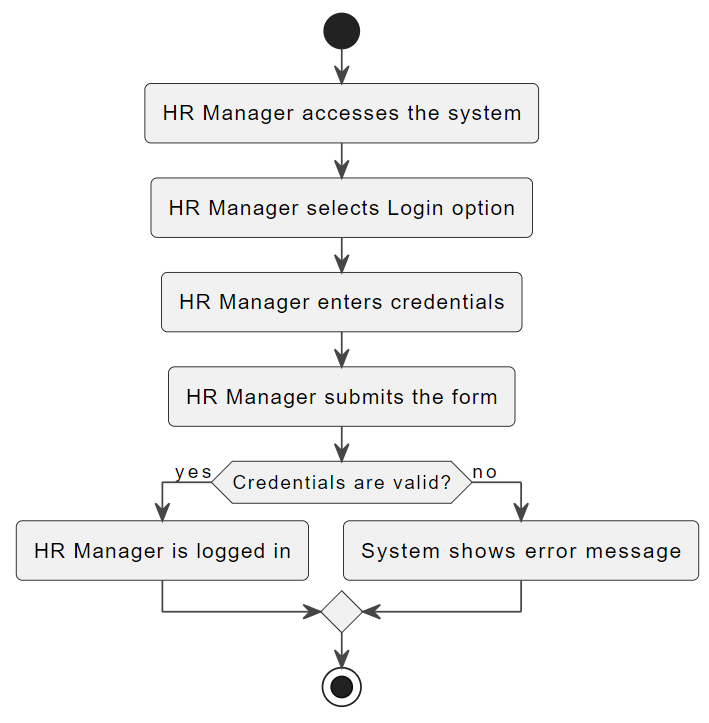
\includegraphics[width=\linewidth]{src/assets/images/sprint1UseCase2ActivityDiagram.PNG}}
    \caption{ Activity Diagram for the Log into the System Use-Case }
    \label{fig:UseCase2_Activity_Diagram}
\end{figure}

\subsection*{Description}
This diagram shows the actions that an HR Manager would take to log into the system. It starts with the HR Manager providing login credentials. The system then validates these credentials. If the validation is successful, the HR Manager gains access to the system. If unsuccessful, an error message is displayed.


\subsubsection{Use Case 3 : Update Profile} 

\begin{figure}[H]
    \centering
    \makebox[\textwidth]{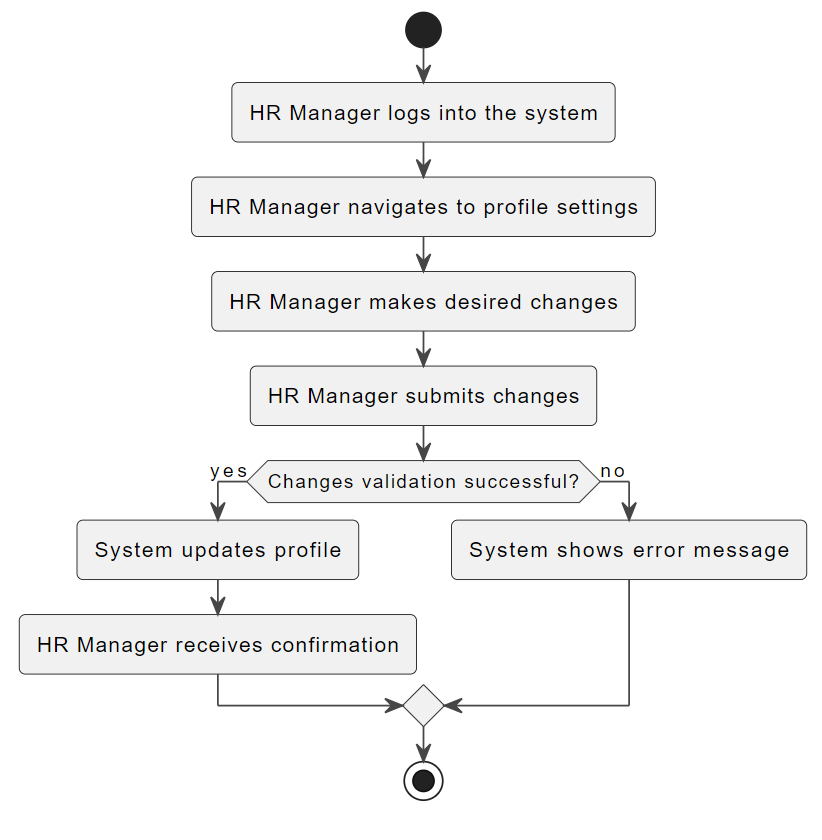
\includegraphics[width=\linewidth]{src/assets/images/sprint1UseCase3ActivityDiagram.PNG}}
    \caption{ Activity Diagram for the Update Profile Use-Case }
    \label{fig:UseCase3_Activity_Diagram}
\end{figure}

\subsection*{Description}
The activity diagram illustrates the sequence of actions for updating a profile. The HR Manager logs into the system, navigates to profile settings, makes the desired changes, and submits them. The system then validates the changes. If the validation is successful, the profile is updated and a confirmation message is shown. If unsuccessful, an error message is displayed.

\subsection{Detailed Sequence Diagrams}
Sequence diagrams provide a detailed visual representation of interactions among different entities in the system, outlining how processes operate with one another and in what order. They are essentially a graphical depiction of an exchange of information between entities over time. In the context of our system, sequence diagrams allow us to trace the sequence of events and operations that take place during the execution of a use case.

In the following sections, we present the sequence diagrams corresponding to the user stories in our first sprint. These diagrams clearly showcase the interactions between the user and the system, displaying the series of actions that occur from the start to the end of a specific scenario. By focusing on the temporal sequence of the messages exchanged between the system and the users, these diagrams provide a deep insight into the overall system behavior for each use case.

\subsubsection{Use Case 1: Sign Up and Create Profile} 


\begin{figure}[H]
    \centering
    \makebox[\textwidth]{\includegraphics[width=1.25\linewidth]{src/assets/images/SD-Signup-Create-Profile.jpg}}
    \caption{ Sequence Diagram for the Sign Up and Create Profile Use-Case }
    \label{fig:UseCase1_Sequence_Diagram}
\end{figure}

\newpage
\subsection*{Description}

The sequence diagram adds further depth to the activity diagram by showcasing the detailed interaction between the prospective HR Manager and the system components, including the Firebase Authentication, Firestore database, and page redirections, all tied together in an interconnected system.

The diagram begins with the user accessing the system and choosing a category, which in the case of the HR Manager is 'Companies/Organizations'. After this selection, the user chooses to create an account, starting an intricate sequence of request-response patterns between the user and the system.

The first interaction includes creating an account through Firebase Authentication, generating a new user document in the Firestore database and subsequently creating a profile document linked to this user. This process necessitates a consistent interaction between the system and Firebase services, manifesting in the form of a series of requests from the system to Firebase and back.

Simultaneously, the system carries out actions to update the user's document with the chosen category and the created profile reference. After successfully creating the account and setting up the profile document, the system directs the user to a page specifically designed for their chosen category to complete their profile.

The diagram encapsulates the entire process of account creation, profile setup, and redirection to the profile page, each step comprising of a request from the user (or system in the case of auto-generated actions) and a response from the system or Firebase services, up to the completion of the profile creation process.

This updated description takes into account the additional details provided in the enhanced sequence diagram, including the specific interactions with Firebase Authentication and Firestore services, and the handling of user categories and profile references.


\subsubsection{Use Case 2: Log into the System} 


\begin{figure}[H]
    \centering
    \makebox[\textwidth]{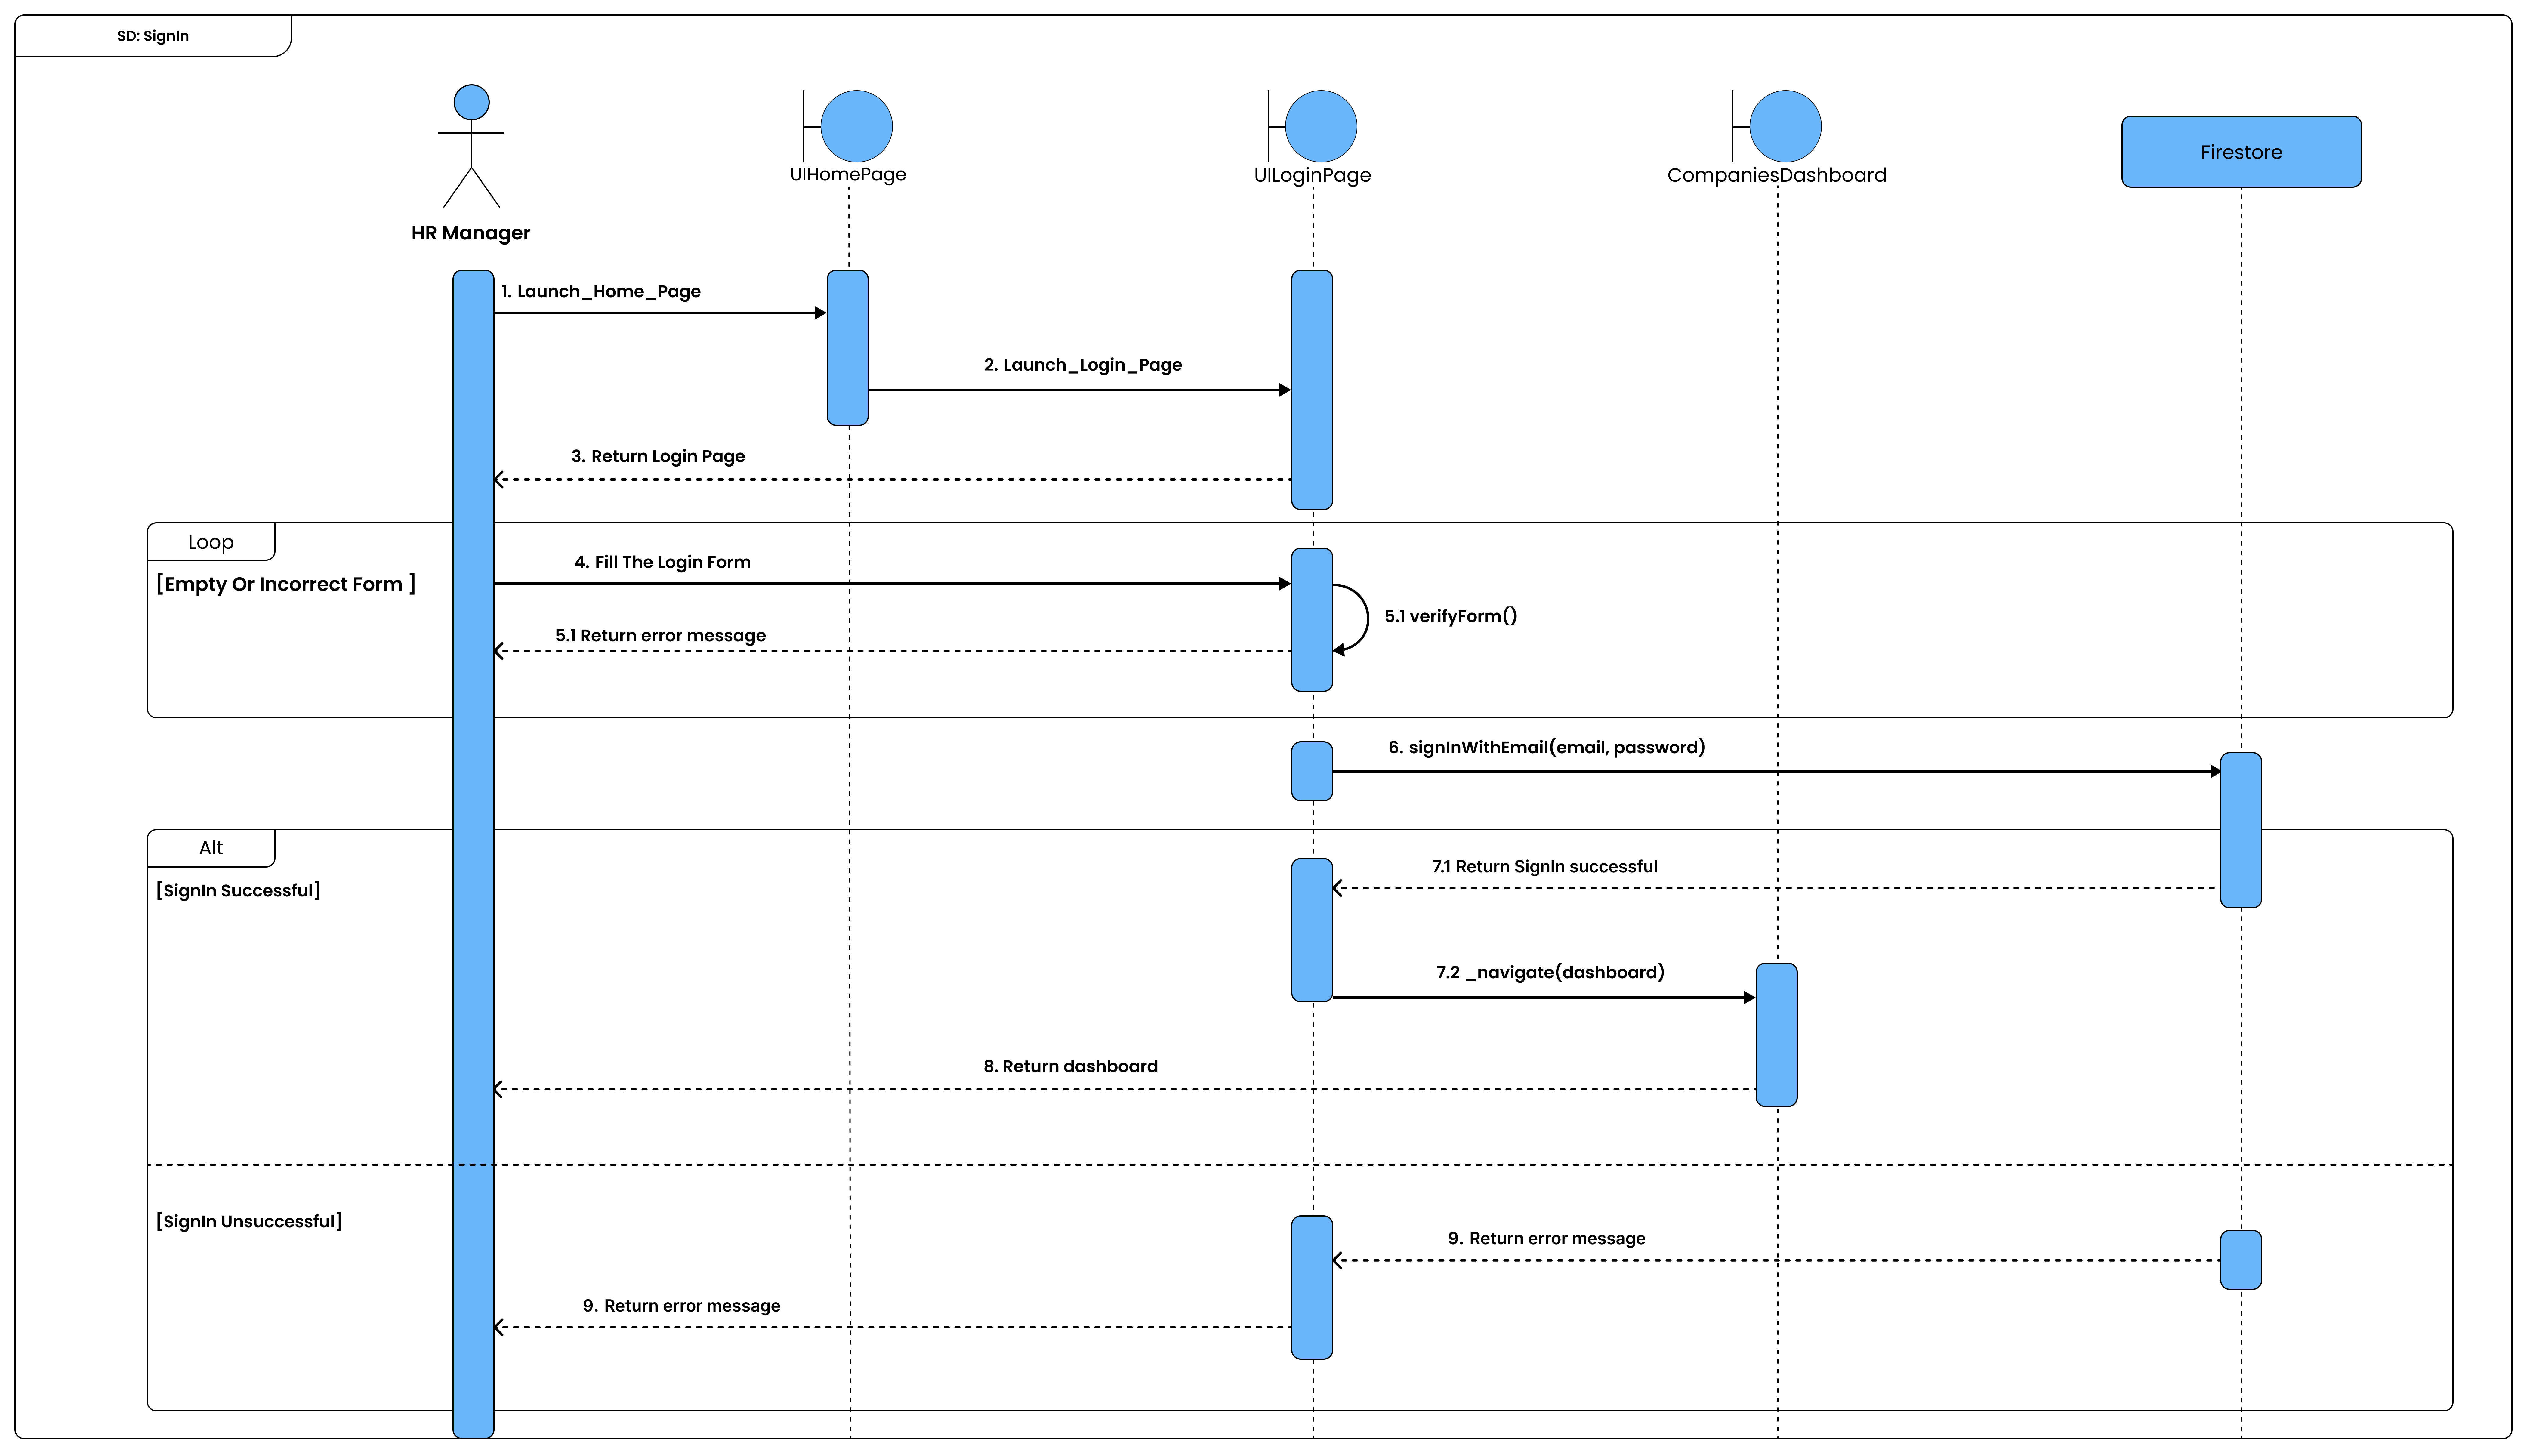
\includegraphics[width=1.25\linewidth]{src/assets/images/SD-SignIn.jpg}}
    \caption{ Sequence Diagram for the Log into the System Use-Case }
    \label{fig:UseCase2_Sequence_Diagram}
\end{figure}

\subsection*{Description}
The sequence diagram demonstrates the detailed exchange between the HR Manager and the system components, namely Firebase Authentication and Firestore database, during the login process. It initiates with the HR Manager's intent to login, followed by the system's validation of login credentials against the data stored in Firebase.

A key consideration here is the user category, which influences the page the user will be directed to upon successful login. Therefore, the diagram also encapsulates the system's verification of the user category and subsequent redirection to the relevant page.

In case of unsuccessful login, due to incorrect credentials or an attempt to log in from an unsuitable category, the system provides appropriate error messages to guide the user. This updated description thus offers an in-depth understanding of the login process including authentication, user category verification, and redirection.

\subsubsection{Use Case 3 : Update Profile} 
\begin{figure}[H]
    \centering
    \makebox[\textwidth]{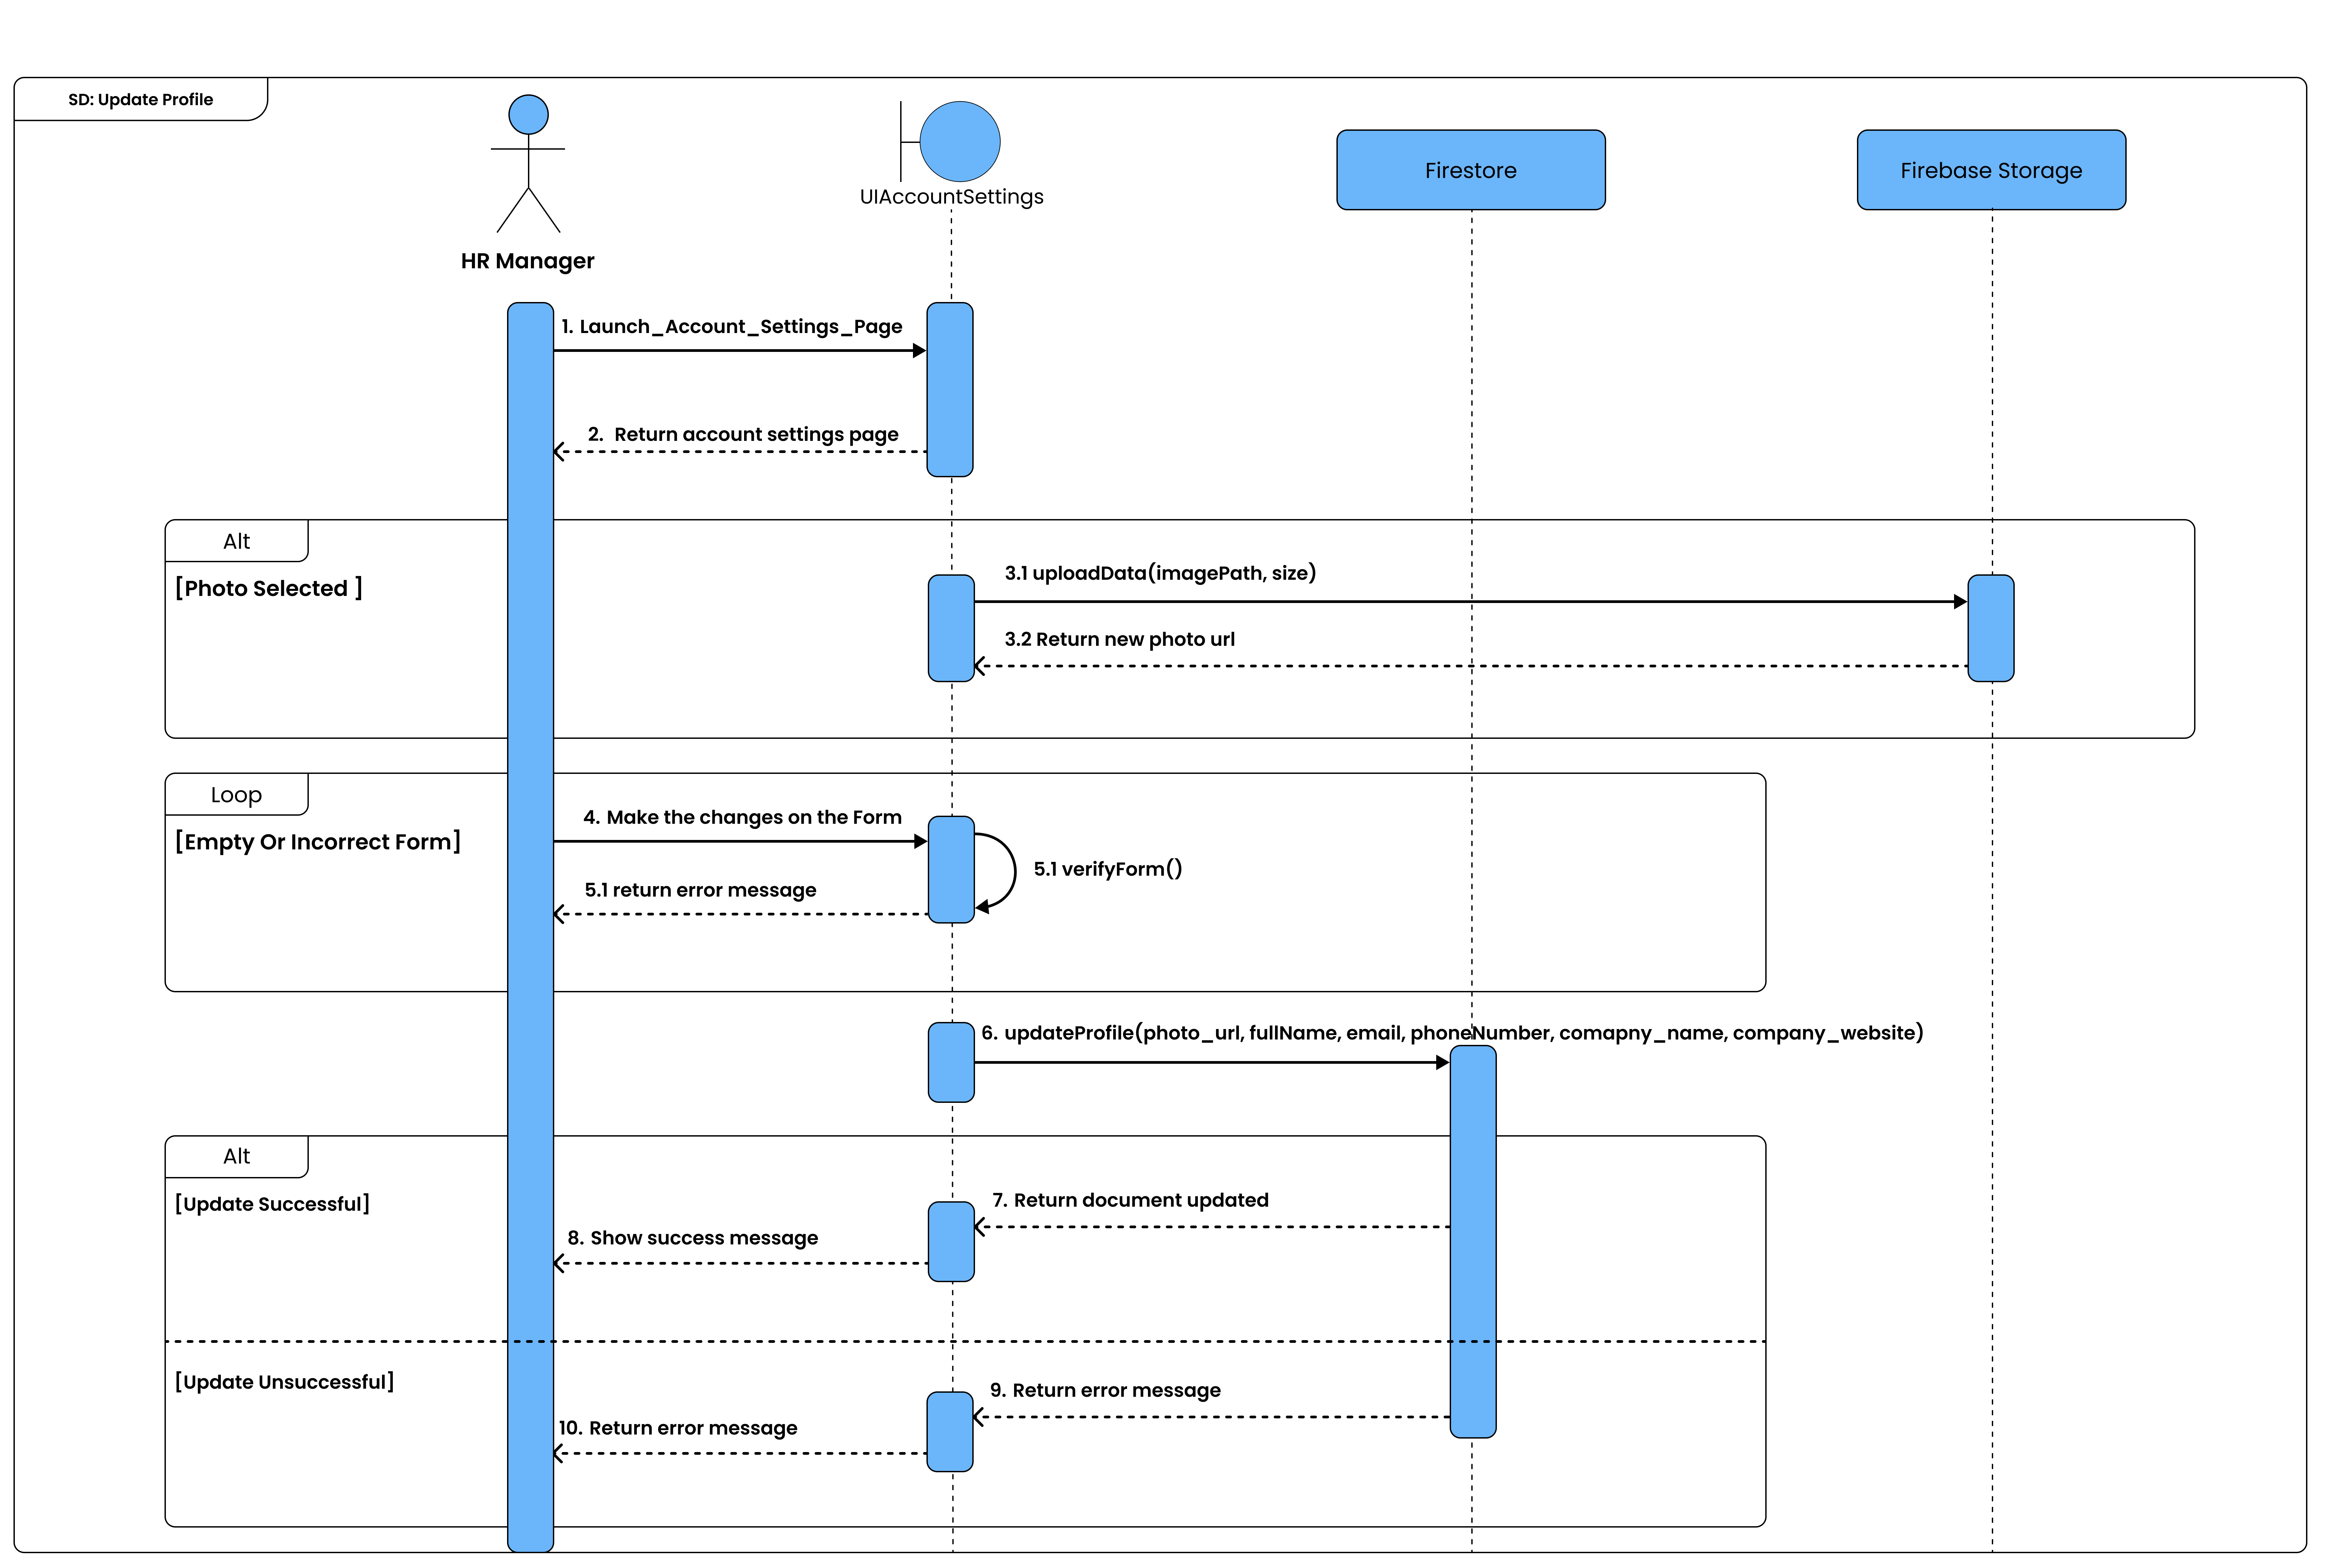
\includegraphics[width=1.25\linewidth]{src/assets/images/SD-Update-Profile.jpg}}
    \caption{ Sequence Diagram for the Update Profile Use-Case }
    \label{fig:UseCase3_Sequence_Diagram}
\end{figure}

\subsection*{Description}
The sequence diagram offers an in-depth view of the interaction between the HR Manager and the system during the profile update process, highlighting the system's connection with Firebase Firestore for data update and Firebase Storage for media upload.

This diagram illustrates how the HR Manager accesses account settings, chooses to update their profile, uploads new profile picture to Firebase Storage (if desired), and submits the new data. It shows a series of conditional actions, one for a regular update of textual information and another for photo upload, which are consolidated upon the user pressing the 'Update' button.

The updated data, whether textual information or a new profile photo, is then stored in Firestore, and the system refreshes the page to reflect the changes. This description, therefore, highlights the multi-faceted nature of the profile update process and how the system interacts with different Firebase services to achieve it.


\section{Implementation}
In the first sprint, the main goal was to establish system access and user profile management. This involved creating functionalities for users to sign up, log in, and manage their profiles.

\subsection{Sign Up and Profile Creation} 

The first step was to design and implement the sign-up process. This involved creating a sign-up page with the necessary fields such as name, email, password, and company details.

The backend functionality was then developed to register and store the new user's data in the database by setting up the database schema and writing the necessary server-side code to handle the registration process.

\begin{figure}[H]
    \centering
    \makebox[\textwidth]{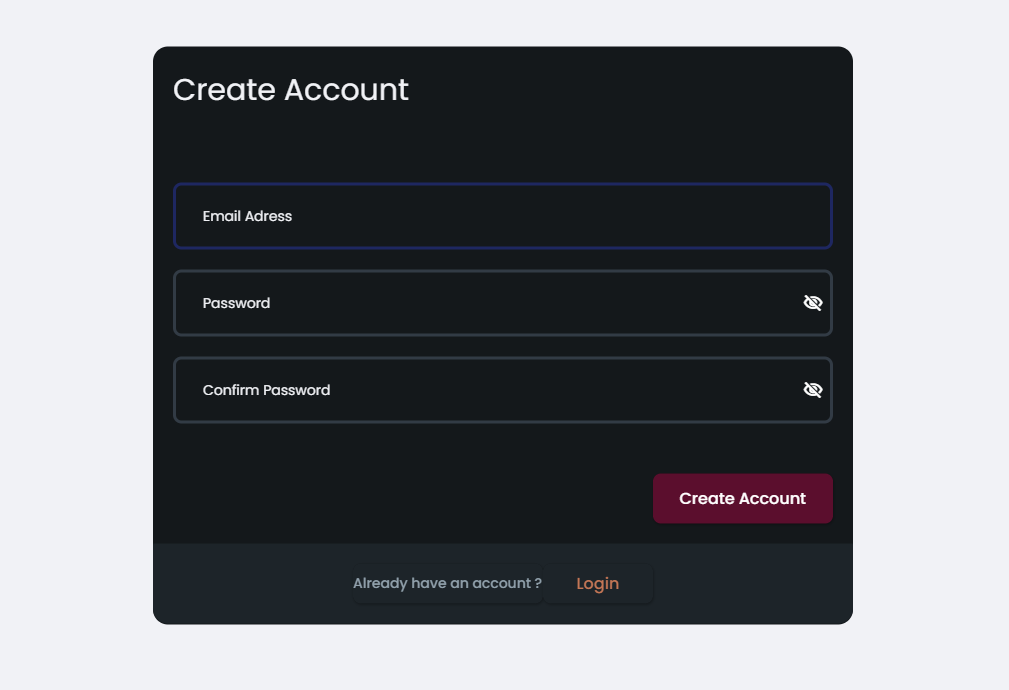
\includegraphics[width=0.9\linewidth]{src/assets/images/sprint1_SignUp.PNG}}
    \caption{ Sign-Up Interface overview page}
    \label{fig:Sign-Up-Interface-overview-page}
\end{figure}

\begin{figure}[H]
    \centering
    \makebox[\textwidth]{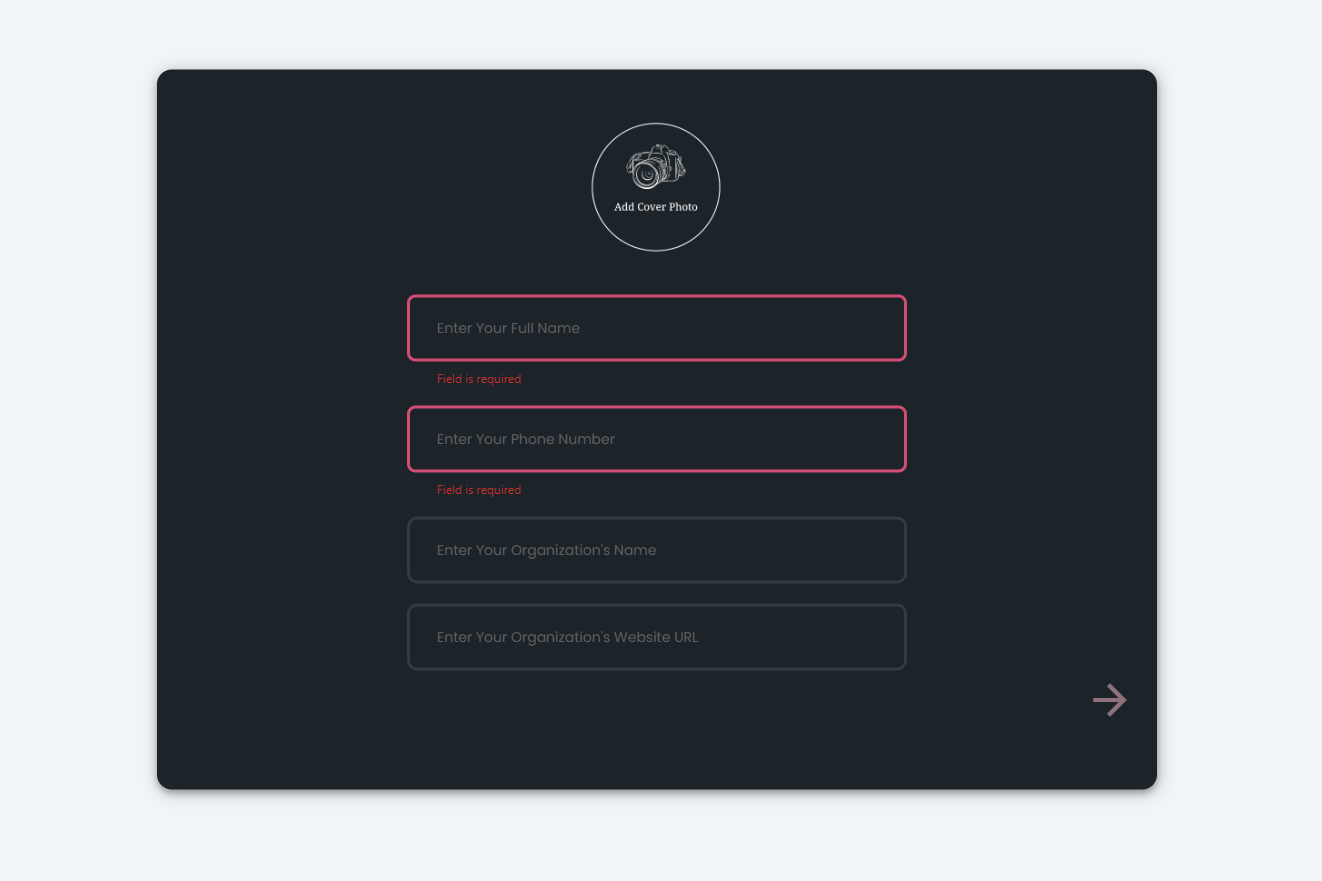
\includegraphics[width=\linewidth]{src/assets/images/sprint1-profile1.PNG}}
    \caption{ Create Profile First Interface overview page}
    \label{fig:Create-Profile-First-Interface-overview-page}
\end{figure}

\begin{figure}[H]
    \centering
    \makebox[\textwidth]{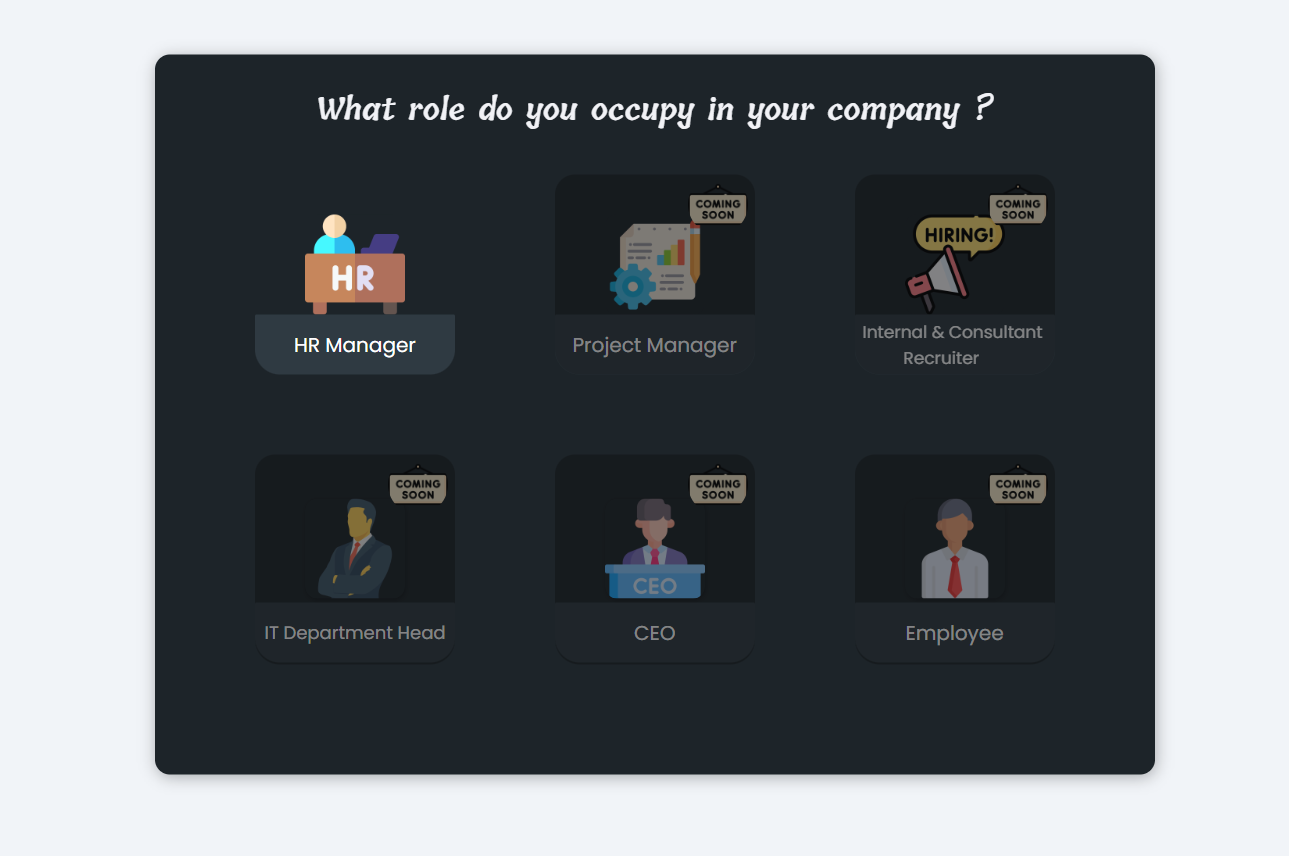
\includegraphics[width=\linewidth]{src/assets/images/sprint1-profile2.PNG}}
    \caption{ Create Profile Second Interface overview page}
    \label{fig:Create-Profile-Second-Interface-overview-page}
\end{figure}


\subsection{Login}

The next step was to design and implement the login process. This involved creating a login page where users could enter their credentials (username/email and password).

The backend functionality was then developed to authenticate the user's credentials and grant access to the system. This involved writing server-side code to check the provided credentials against the stored user data in the database.

\begin{figure}[H]
    \centering
    \makebox[\textwidth]{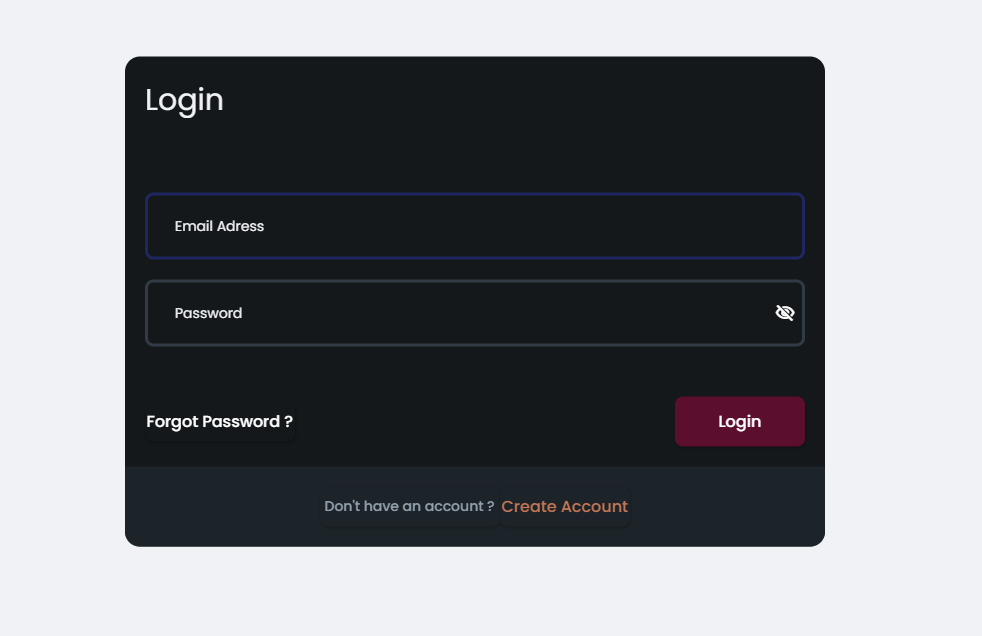
\includegraphics[width=\linewidth]{src/assets/images/sprint1_LogIn.PNG}}
    \caption{ Sign-In Interface overview page}
    \label{fig:Sign-In-Interface-overview-page}
\end{figure}



\subsection{Profile Management}

The final step was to develop a feature that allows users to update their profile information or delete their account. This involved creating an account settings page where users could view and edit their profile details.

The backend functionality was then developed to handle these updates and deletions. This involved writing server-side code to update or delete the user's data in the database based on their input.


\begin{figure}[H]
    \centering
    \makebox[\textwidth]{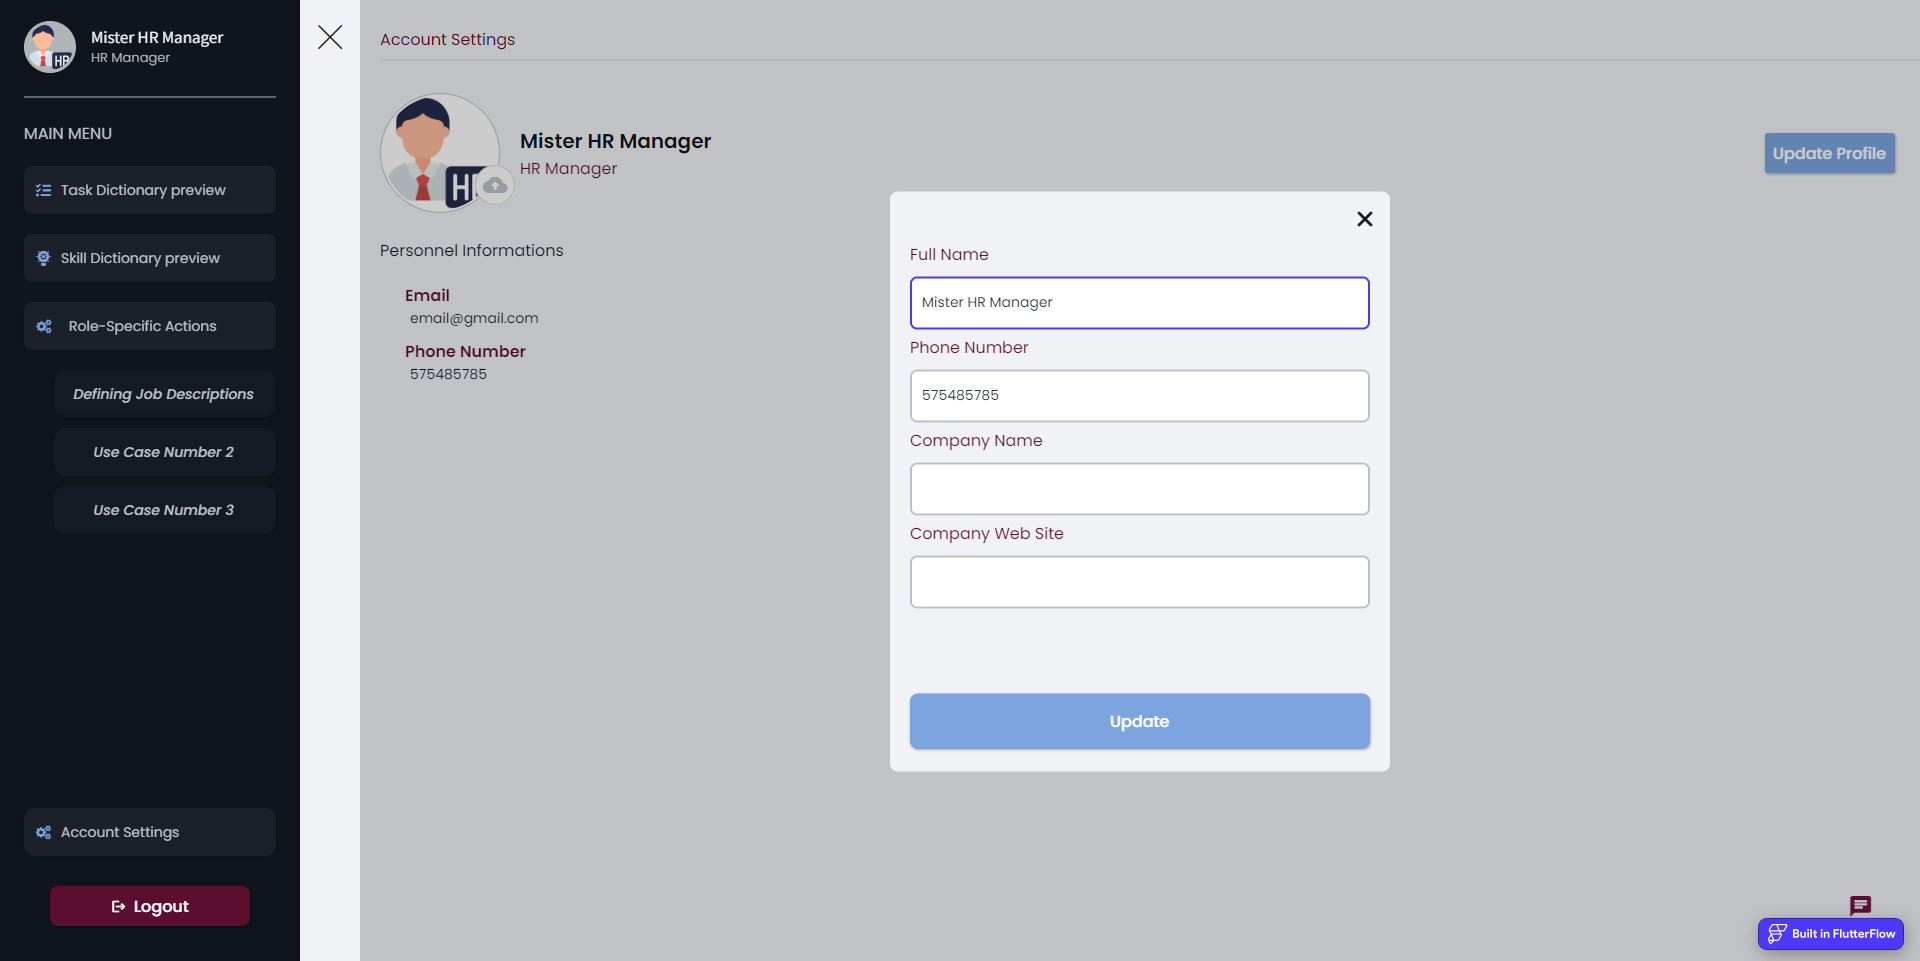
\includegraphics[width=\linewidth]{src/assets/images/sprint1_AccountSettings.PNG}}
    \caption{ Account Settings Interface overview page}
    \label{fig:Account-Settings-Interface-overview-page}
\end{figure}


\subsection{Integration}

Once all these features were developed, they were integrated into the overall system. This involved ensuring that they interacted correctly with other system features and data, and that they provided a smooth and intuitive user experience.

\subsection{Testing}

Finally, thorough testing was conducted to ensure that all the features worked as expected. This involved testing each feature individually and as part of the overall system, and fixing any bugs or issues that were identified.



% ----------------------------------- SECTIONS (^) ----------------------------------- %
